\subsection{\glyph{Submap}}\label{sec:submap}

A \glyph{submap} is used to encapsulate a map (including all types of nodes and edges) within one glyph.
As such, it is not equivalent to an \glyph{omitted process} (\sect{omitted}).
The \glyph{submap} hides the content of this map to the users, and displays only \glyph{submap terminals} (\sect{submapTerminal}).
In the case of an SBGN description that is made available through a software tool, the map enclosed by the  \glyph{submap} may be available to the tool.
A user could then ask the tool to expand this map in a different canvas, for instance by clicking on the \glyph{submap}.
In the case of an SBGN description made available in a book or a website, the content of the map may be available on another page, possibly accessible via an hyperlink on the \glyph{submap}.

\begin{glyphDescription}

\glyphSboTerm
SBO:0000395 ! encapsulating process

\glyphIncoming
None.

\glyphOutgoing
None.

\glyphContainer
A \glyph{submap} is represented by a rectangular shape, to remind that it is fundamentally a process.

\glyphLabel
A \glyph{submap} is identified by a label that is an unbordered box containing a string of characters.
The characters may be distributed on several lines to improve readability.
The centre of the label must be placed on the centre of the shape.
The label may extend outside of the shape.

\glyphAux
A \glyph{submap} must carry one or more \glyph{submap terminals} (\sect{submapTerminal}), each linked to an \glyph{EPN} (\sect{EPNs}) or \glyph{compartment} (\sect{compartment}) of the map using an \glyph{equivalence arc} (\sect{equivalenceArc}).

\end{glyphDescription}

\begin{figure}
\begin{center}
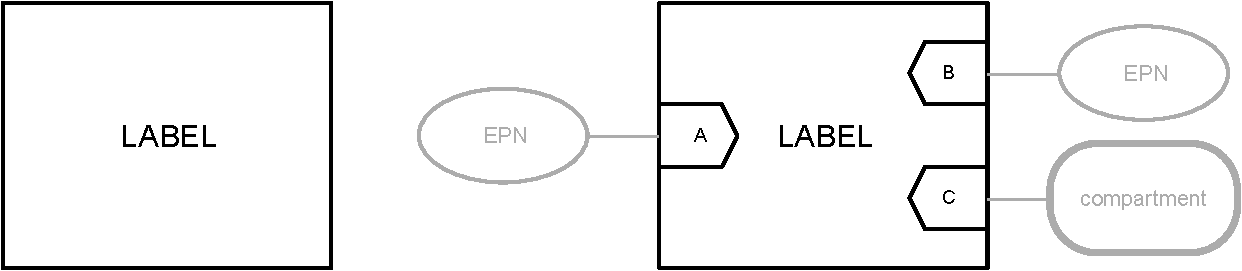
\includegraphics[scale=0.7]{images/build/submap.pdf}
\caption{The \PD glyph for \glyph{submap}, shown plain and unadorned on the left, and with three \glyph{submap terminals} on the right.}
\label{fig:submap}
\end{center}
\end{figure}

\fig{folded} represents a \glyph{submap} that encapsulates processes transforming glucose into fructose-6-phosphate.
The \glyph{submap} carries five \glyph{submap terminals}, four linked to \glyph{EPNs} and one linked to a \glyph{compartment}.
The latter is particularly important in the case of \glyph{EPNs} present only in a \glyph{compartment} enclosed in a \glyph{submap}, and that are not linked to \glyph{submap terminals} themselves.
Note that the \glyph{submap terminals} do not allow defining a ``direction'' for the flux of the processes enclosed in the \glyph{submap}, which is solely determined by the context as in \fig{folded}.

\begin{figure}
\begin{center}
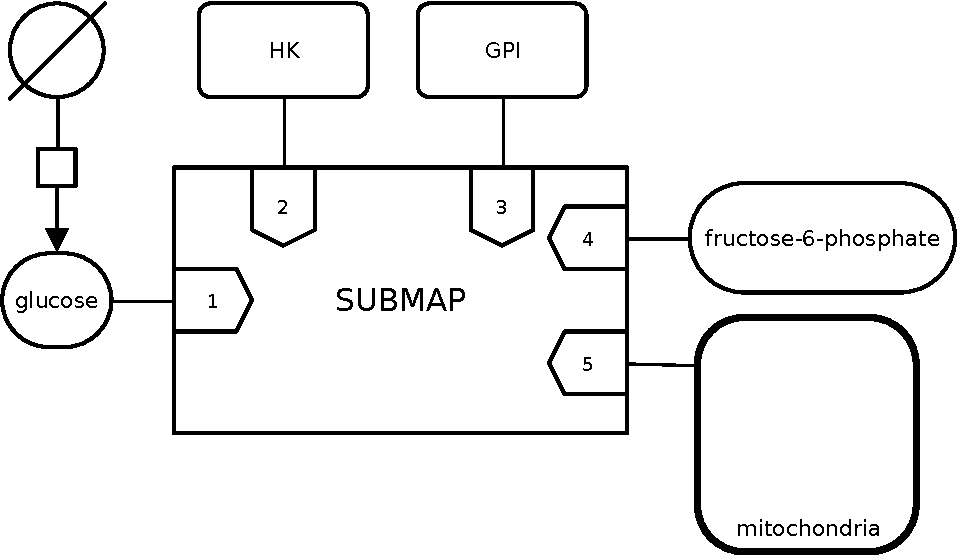
\includegraphics[scale=0.8]{images/build/submap_folded_example.pdf}
\caption{Example of a \glyph{submap} encapsulating processes that transform glucose into fructose-6-phosphate.
The map enclosed by the \glyph{submap} is shown in \fig{unfolded}, whose \glyph{tags} are referred to by the \glyph{submap terminals} decorating the present \glyph{submap} glyph.
}
\label{fig:folded}
\end{center}
\end{figure}

The map in \fig{unfolded} represents the map enclosed in the \glyph{submap} of \fig{folded}.
Note that the tag 5 links the mitochondria \glyph{compartment} in this map to the mitochondria \glyph{compartment} of the main map in \fig{unfolded}.

The \glyph{compartment} containing glucose-6-phosphate is implicitly defined as the same as the \glyph{compartment} containing glucose and fructose-6-phosphate.
There is no ambiguity because if glucose and fructose-6-phosphate were in different \glyph{compartments}, at least one of them would have been linked to a \glyph{submap terminal} of the \glyph{submap} of \fig{folded}.

\begin{figure}
\begin{center}
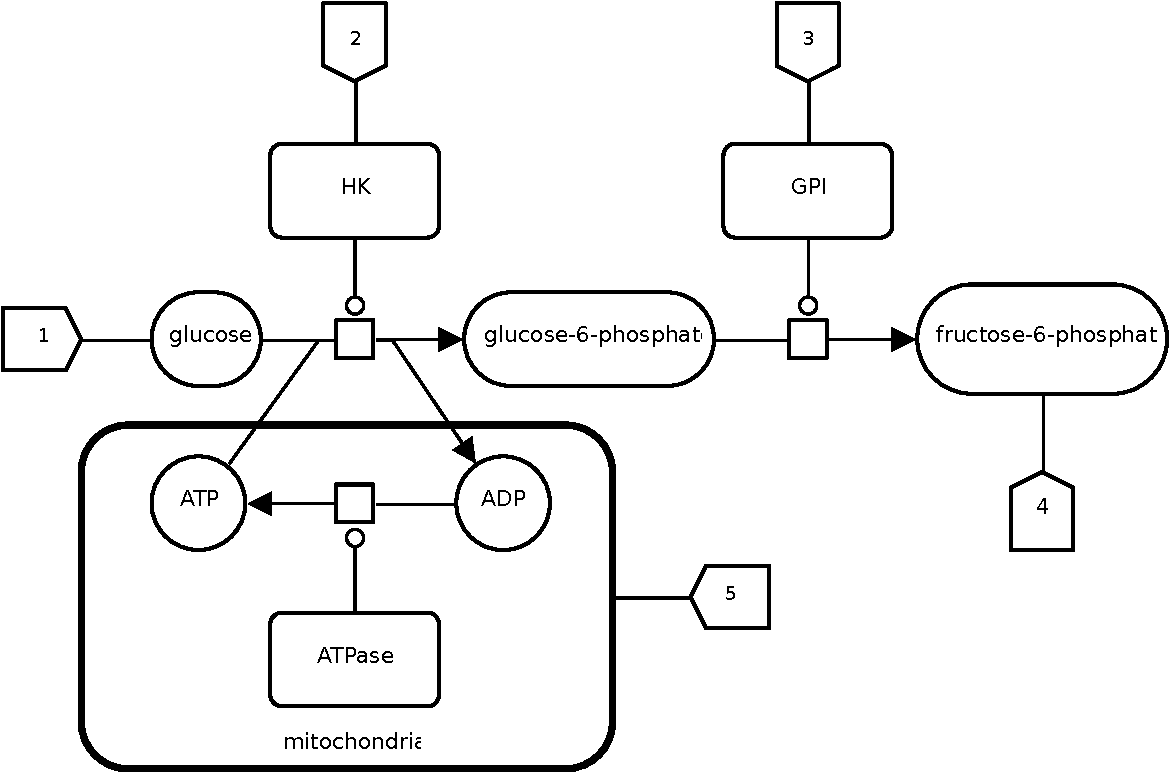
\includegraphics[scale=0.8]{images/build/submap_unfolded_example.pdf}
\caption{Example of a map with \glyph{tags}, showing that it is enclosed in a \glyph{submap} of another map (here, the one of \fig{folded}).}
\label{fig:unfolded}
\end{center}
\end{figure}
